\documentclass[12pt]{article}
\usepackage{float}
\usepackage{graphicx}
\usepackage{minted}
\usepackage{amsmath}
\usepackage[
backend=biber,
style=numeric,
sorting=ynt
]{biblatex}
\pagenumbering{gobble}		% Research.gov wants no page numbering
\tolerance9000

\usepackage[letterpaper,margin=1in]{geometry}
\renewcommand{\footnotesize}{\small\spaceskip4pt plus1.5pt}

\addbibresource{convex_hull.bib}
\nocite{*}

\author{Claudia Cortell (ccc2223), Kyle Edwards (kje2115), and Avighna Suresh (as6469)}
\title{Parallel Convex Hull : Project Proposal}

\begin{document}

\maketitle

% \centerline{\bf Parallel Convex Hull Project Proposal}
\setcounter{section}{0}

\section{Motivation}


Given a set P of n points in a plane, the convex hull of P is the smallest convex polygon containing the points and the largest convex polygon whose vertices are points in P. Finding the convex hull of a set of points has many applications in various fields, some of the more notable examples being generating simplified 3D meshes, performing collision detection between complicated objects, extracting shapes for image processing, and pathfinding.

\begin{figure}[h]
	\centering
	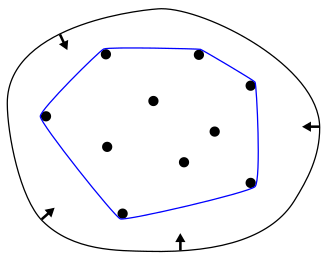
\includegraphics[width=0.5\textwidth]{convex_hull.png}
	\caption{a good analogy for a 2d convex hull is to imagine a rubber band
		enveloping the points.}
\end{figure}

Due to the large number of use cases for convex hulls and the relative lack of already existing parallel algorithms for the problem, our project aims to parallelize an existing convex hull algorithm. Specifically, we aim to implement both a sequential and parallel convex hull algorithm in order to compare the increase in speed that parallelization would provide.

%%%%%%%%%%%%%%%%%%%%%%%%%%%%%%%%%%%%%%%%%%%%%%%%%%%%%%%%%%%%%%%%%%%%%%%%%%%%%%%%
\section{Algorithms}

For the remainder of the proposal, we will define constants as such: $n$ denotes the number of input points, $h$ denotes the number of points on convex hull of the points, $K$ denotes the number of subsets to that will be operated on in parallel, and $m$ denotes the average number of points allocated to each subset, where $m = \frac{n}{K}$.

\subsection{Sequential}


For our sequential convex hull algorithm, we will be using the Graham Scan algorithm, as it is a simple yet effective algorithm that has little volatility in runtime. This algorithm is performed in two stages: ordering the points based on angle, and traversing through the points in order to figure out which point lies on the convex hull. For ordering, a point’s angle is defined as the angle formed between $\hat{i}$ and the vector connecting the point with the lowest $y$ value in the set to the point. The traversal stage uses a stack in order to find the points that lie on the hull: for each point, pop from the stack until the angle formed between the two topmost points and the current point is leftwards, then push the point to the stack. Once all points have been iterated through, all points that remain on the stack are part of the convex hull. Due to the comparison-based sorting, the algorithm’s time complexity is $O(n\log n)$.

\subsection*{Graham Scan Code}

The following code is written in Python.

\begin{minted}{python}
  
def graham_scan(points):
  #Find the lowest y point as the starting point
  p_min = point_with_min_y(points)

  #Sort the points by the angle made by \hat{i} -> p0 -> p
  points = sort_points_by_angle(p0, points)

  #Convex hull
  convex_hull = points[:2]

  #Iterate through the sorted points to create the hull
  for p in points[2:]:
    #Pop from hull until the top 2 points on the hull and the new point 
    #form a counterclockwise (left) turn
    while len(convex_hull) > 1 
          and not is_left_turn(convex_hull[-2], convex_hull[-1], p):
      convex_hull.pop()
    
    convex_hull.append(p)
  
  return convex_hull

\end{minted}

Another sequential algorithm worth mentioning for calculating a convex hull is the Jarvis March (Gift Wrapping) algorithm. This algorithm can be thought of as a much simpler but less efficient version of the Graham Scan algorithm: it chooses the point with the lowest $y$ coordinate, iterates through each point to find the rightmost point angle-wise, adds that point to the list of points on the convex hull, and then repeats this process with the newly added point until the original point is reached. This algorithm has a time complexity of $O(nh)$, though its simplicity makes it good for smaller data sets where $h\leq\log n$.


\section{Parallel}


For the algorithm we plan to parallelize, we have two algorithms we want to parallelize: the Quickhull algorithm, and Chan’s algorithm. To be more specific, Chan’s algorithm requires us to implement Quickhull regardless, so we figure we will first implement Quickhull in a parallel fashion, strip it down to its sequential version, then implement Chan’s algorithm using the sequential version of Quickhull. If this approach is too ambitious, we will stick to just Quickhull.

The Quickhull algorithm is a divide-and-conquer algorithm that recursively partitions the points, removing points that cannot lie on the convex hull with each recursive step. More specifically, the algorithm finds the maximum and minimum points based on their $x$ value, draws a line between them, partitions the points based on which side of the line they lie on, figures out the two points on each side furthest from the line, draws a triangle between that furthest point and the line, removes all points within the triangle, and recurses using the two lines drawn to create the triangle. The time complexity of Quickhull is $O(n \log n)$ when run sequentially, though in the worst-case scenario it has a runtime of $O(n^2)$.

\begin{figure}[h]
	\centering
	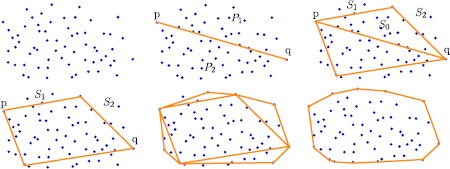
\includegraphics[width=0.75\textwidth]{quickhull.png}
	\caption{A visual representation of the Quickhull steps described previously.}
\end{figure}

Chan’s algorithm is faster than both Quickhull and Graham scan, as it has a time complexity of O(n log h) rather than O(n log n). Similar to Quickhull, the algorithm uses divide-and-conquer: the points are first partitioned into K subsets with m elements each, the convex hull of each subset is found using any $O(n log n)$ convex hull algorithm (we will likely use Quickhull, as unlike Graham Scan, Quickhull can be extended to more than two dimensions), and finally the convex hull of each subset is merged into a final convex hull. The trick lies in how that merging takes place, as it uses a modified version of the gift-wrapping algorithm that only iterates through points that are part of the convex hulls of the subsets.

\begin{figure}[h]
	\centering
	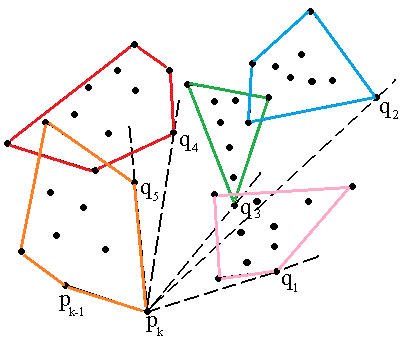
\includegraphics[width=0.5\textwidth]{chans.png}
	\caption{An example of a set split into subsets for Chan's algorithm. Notice that the subsets can have overlapping convex hulls.}
\end{figure}

\subsection*{Quickhull Code}

\begin{minted}{python}

def quick_hull_(points, p1, p2):
  # Base caseif
  if len(points) < 2:
    return points | {p1}

  # Positive distance = to the right of line p1 -> p2
  p_max = max(points, key=lambda p:dist(p, (p1, p2))

  # Remove all points inside the triangle 
  # All points inside triangle are to the left of lines
  # p1 -> p_max and p_max -> p2
  points = points - {[p for p in points 
                      if dist(p,Line(p1,p_max)) < 0 
                      and dist(p_max, p2) < 0]}

  return quick_hull_(points, p1, p_max) | quick_hull_(points, p_max, p2)

def quick_hull(points):
  p_min = min(points, key=lambda p:p.y) 
  p_max = max(points, key=lambda p:p.x)

  return quick_hull_(points, p_min, p_max) ++ quick_hull_(points, p_max, p_min)
\end{minted}

\section{Approach}


Due to its nature as a divide-and-conquer algorithm, parallelization of the Quickhull algorithm will not be too difficult. The simplest approach to parallelization is to perform Quickhull sequentially until there are $K$ lines, then assigning each thread one of the $K$ lines to continue with. The two main issues with this approach are figuring out the optimal value of $K$, and figuring out schemes for load balancing, as there is no guarantee that the number of points each thread will be assigned will be equal. In the best case scenario, $m$ points would be assigned to each thread. The sequential component has a time complexity of $O(n\log k)$, and the parallel component has an average time complexity of $O(m \log m)$, meaning together the total time complexity should be around $O(n \log n - m(K - 1)\log m)$. This suggests that, beyond just improving performance, parallelism using the method described is also less time complex!

Parallelization of Chan’s algorithm is, surprisingly, somewhat easier than it is with Quickhull: we can just assign the task of finding the convex hull of one of the $K$ subsets to a thread each. The largest issue we will run into will be, again, figuring out the optimal value of $m$, which also affects the optimal value of $K$. One suggested method we found is the so-called squaring method: at each recursive iteration $t$ of the algorithm (we previously only described one iteration of the algorithm, but for larger sets we can perform multiple), we choose $m = \text{min}(n, 2^{2^t})$. This results in a maximum depth of $\log(\log(h))$, which altogether results in a time complexity of $O(n\log h)$. Our implementation will use this value of $m$, although it’s unlikely that we will have experiments with more than one iteration, meaning that $m$ will equal 4 in most situations. We will also experiment with other values of $m$, if time permits. Using the Master Theorem, we can conclude that the time complexity of the parallel approach is $O(Kh\log m)$, which for cases where $h \leq m$ gives us a slightly better time complexity than the $O(n\log h)$ time complexity of the sequential version.

On the Haskell side, we will use the Par monad and Strategies in order to parallelize our algorithm. We may also play around with using REPA for Quickhull, as finding the points that lie within a triangle appears to be a good place to use REPA. For input data, we’ll just generate some random points and write them to a file, then read from that file so that we can produce equal test cases. If time permits, we also plan on rendering the resulting convex hull, though this may not necessarily be done in Haskell.

\nocite{*}
\printbibliography

\end{document}
